\documentclass[paper=a4, fontsize=11pt]{scrartcl}
\usepackage{enumerate}
\usepackage{amsmath}
\usepackage{amssymb}
\usepackage{tikz}
\newcommand{\parens}[1]{ \left( #1 \right) }
\begin{document}
\noindent Willy Xiao and Kevin Eskici \\ STAT 221 \\Pset 3\\ Oct 22, 2014
\begin{enumerate}[\text{question }1.]
  \item Show: \\
    \begin{enumerate}[(a)]
      \item \begin{align*}
        E\left[ \nabla l(\theta; y) \right] &= 0 \text{ at }\theta^* \\
        \nabla l(\theta; y) &= \frac{(y - b'(x^T\theta^*))*x}{\phi} \\
        E\left[ \frac{y_n - b'(x^T\theta^*)}{\phi} \right] &= \frac{E(Y) - b'(x^T\theta^*)}{\phi} = 0 \\
        E(Y) &= b'(x^T\theta^*)
      \end{align*}
      \item \begin{align*}
        \text{ We know that } -E\left[ \nabla \nabla l(\theta; y) \right] &= E\left[ \nabla l(\theta; y) \right]^2 \\
        \nabla \nabla l(\theta; y) &= \frac{-b''(x^T\theta^*)}{\phi} \\
        E\left[ \frac{Y - b'(\lambda)}{\phi} \right]^2 &= \frac{E(Y - E(Y))^2}{\phi^2} = \frac{Var(Y)}{\phi^2} \\
        \phi b''(\lambda_n) = \phi h'(\lambda_n) &= var(y_n|\lambda_n)
      \end{align*}
      \item \begin{align*}
        l(\theta; y) &= \frac{\lambda_ny_n - b(\lambda_n)}{\phi} + \log{y_n, \phi} \\
        \nabla l(\theta, y) &= \frac{1}{\phi}*(y_n - b'(x^T\theta))x_n \\
          &= \frac{1}{\phi}*(y_n - h(x^T\theta))x_n
      \end{align*}
      \item This is the fisher's information:
        \begin{align*}
          - \nabla \frac{1}{\phi}*(y_n - h(x^T\theta))x_n &= \nabla \frac{1}{\phi}*h(x^T\theta)x_n \\
          I(\theta) &= \frac{1}{\phi} E(h'(x^T\theta)x_nx_n^T)
        \end{align*}
      \item Because we know the fisher's information must be positive (it's a variance) and we know that $x_nx_n^T$ is positive-definite, then that means $h'(x^T\theta)$ must also be positive. If this is true then it means $h(\cdot)$ is non-decreasing.
    \end{enumerate}
  \item Experiment: \\
    \begin{enumerate}[(a)]
      \item
        \begin{align*}
          \text{ SGD: } \theta_{t+1} &= \theta_t + (1 + .02*t)^{-1}*(\Sigma^{-1}*(\vec{x_t} - \vec{ \theta_t})) \\
          \text{ ASGD: } \overline{\theta}_{t+1} &= (1 - 1/t)*\overline{ \theta }_t + (1/t)*\theta_{t+1} \\
              & \text{ where } \theta_{t+1} = \theta_t + (1 + .02*t)^{-2/3}*(\Sigma^{-1}*(\vec{x_t} - \vec{ \theta_t})) \\
          \text{ ASGD\_BAD: } & \text{ Same as ASGD, but with learning rate } (1 + t)^{-1} \\
          \text{ Implicit: } \theta_{t+1} &= (1 + \gamma_t)^{-1}*(\theta_t + \gamma_t*\vec{x_t}) \text{, where } \gamma_t = (1 + .02*t)^{-1} \\
        \end{align*}
        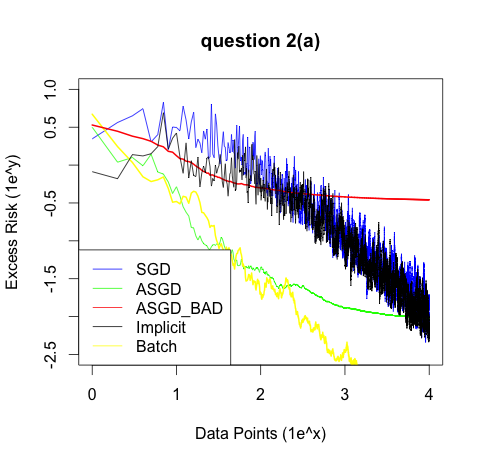
\includegraphics[width=400px]{2a.png}
      \item For SGD and implicit, we use a learning rate $a_t$ of $\gamma_0 * (1 + \gamma_0 \lambda_0 t)^{-1}$ and for ASGD we use $\gamma_0 * (1 + \gamma_0 \lambda_0 t)^{-2/3}$. Where $\gamma_0 = tr(A)$ and $\lambda_0 = .01$. \\
        \begin{align*}
          \text{ SGD: } \theta_{t+1} &= \theta_t - a_t * x^T\theta_tx + a_t * y * x \\
          \text{ ASGD: } \overline{\theta}_{t+1} &= (1 - 1/t)*\overline{ \theta }_t + (1/t)*\theta_{t+1} \\
          \text{ Implicit: } \theta_{t+1} &= \theta_t - a_t f_t x^T \theta_t x + a_t y x - a_t^2 f_t y \Sigma(x^2) x\\
            & \text{ where: } f_t = 1 / (1 + a_t \Sigma(x^2) ) \\
            & \text{ Note: this is taken from Panos' distro code } \\
          \text{ Batch: } & \text{ We ran the linear regression using R's lm(y } \sim \text{ x + 0) } \\
        \end{align*}
        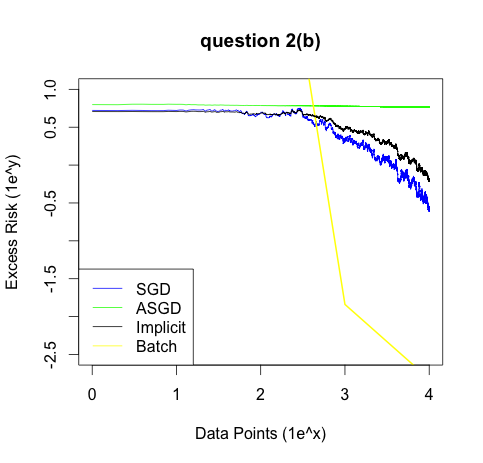
\includegraphics[width=400px]{2b.png}
        Note: After trying multiple learning rates and averaging rates for ASGD, for some reason we were still unable to produce the correct convergence rate. It may be some misunderstanding on our part or simply a bug in the code, but this will affect also 2(c).
      \item We ran our script task2c.slurm. We ran it for $n = {100, 1000, 5000, 10000}$ each at $400$ reps. Then we chose amin to be $51$ and amax to be $100$. All code for this is in task2c\_runner.R. Plots below: \\
        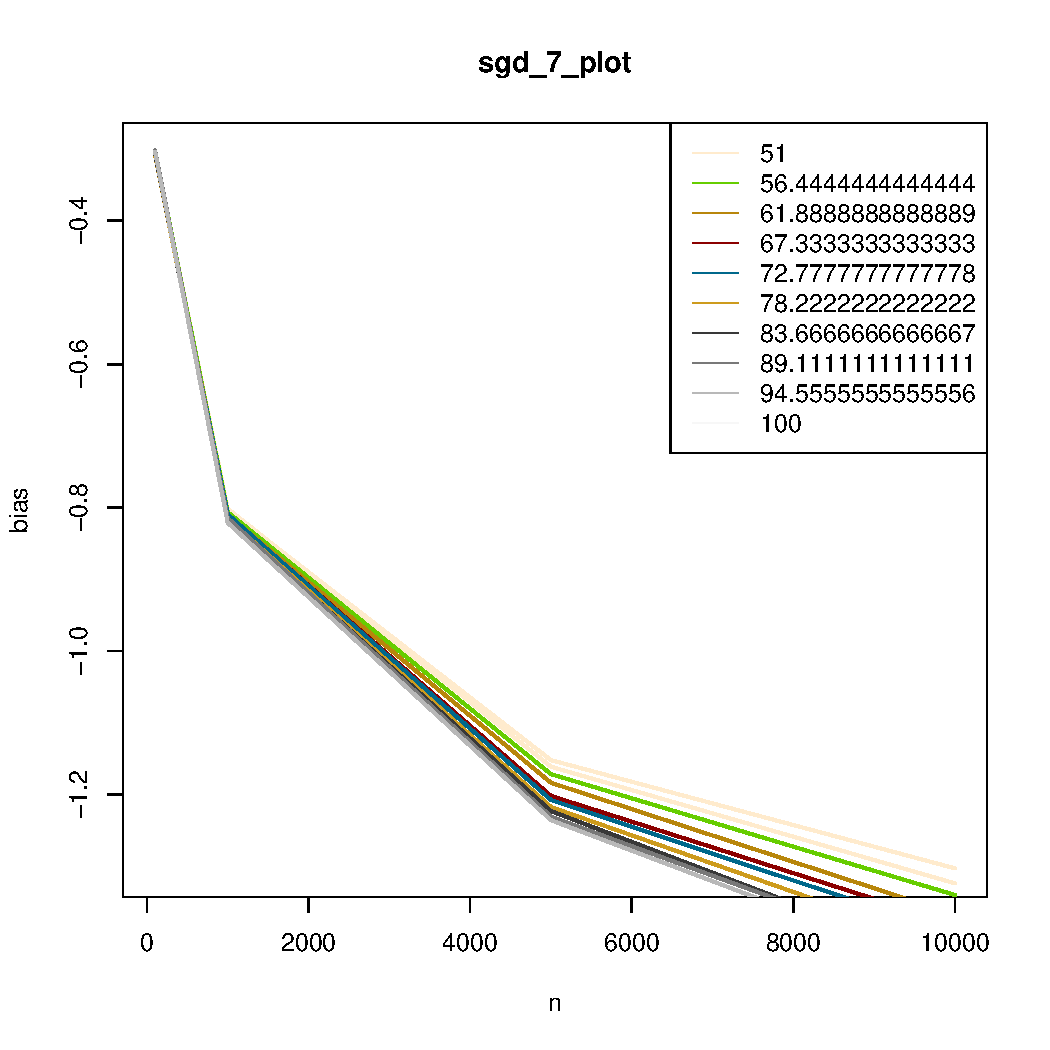
\includegraphics[width=250px]{sgd_7_plot.pdf} \\
        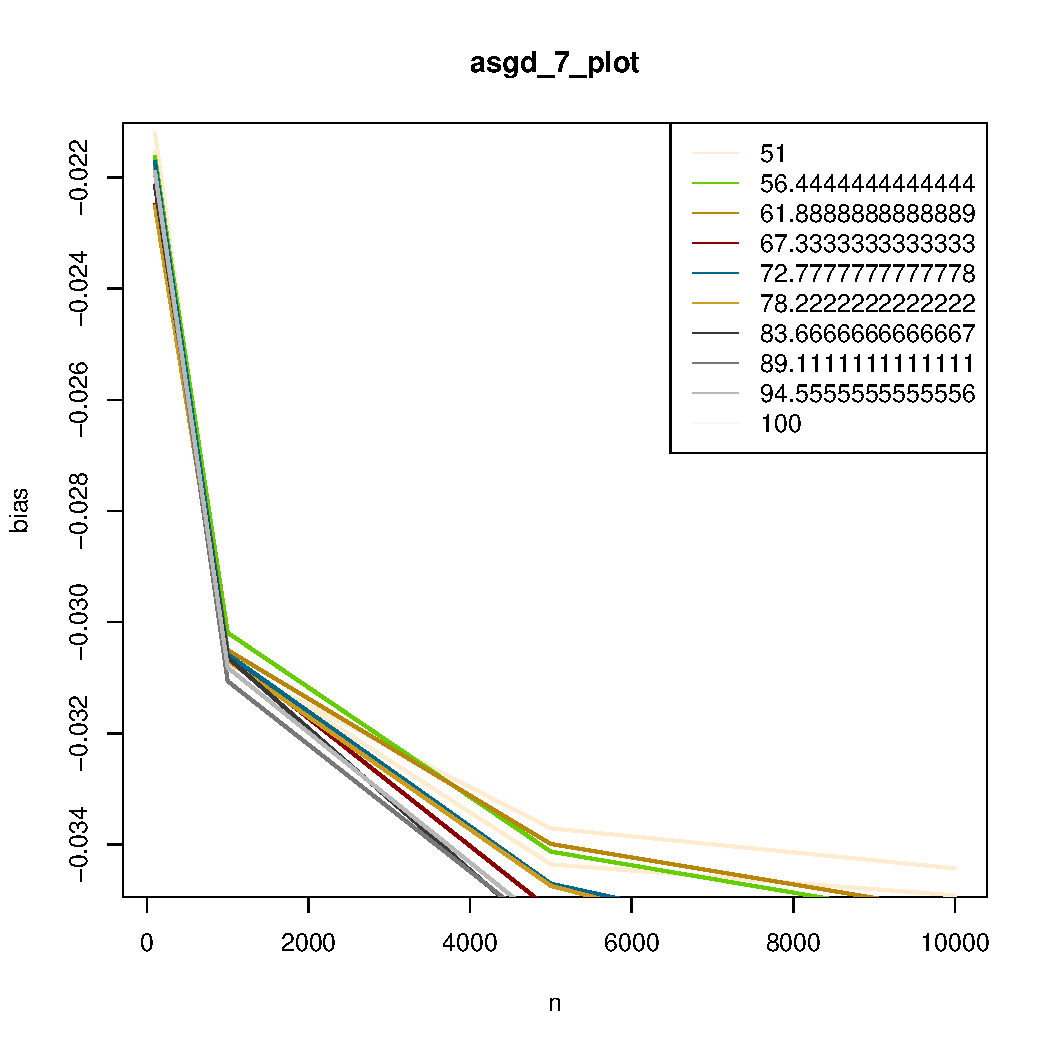
\includegraphics[width=250px]{asgd_7_plot.pdf} \\
        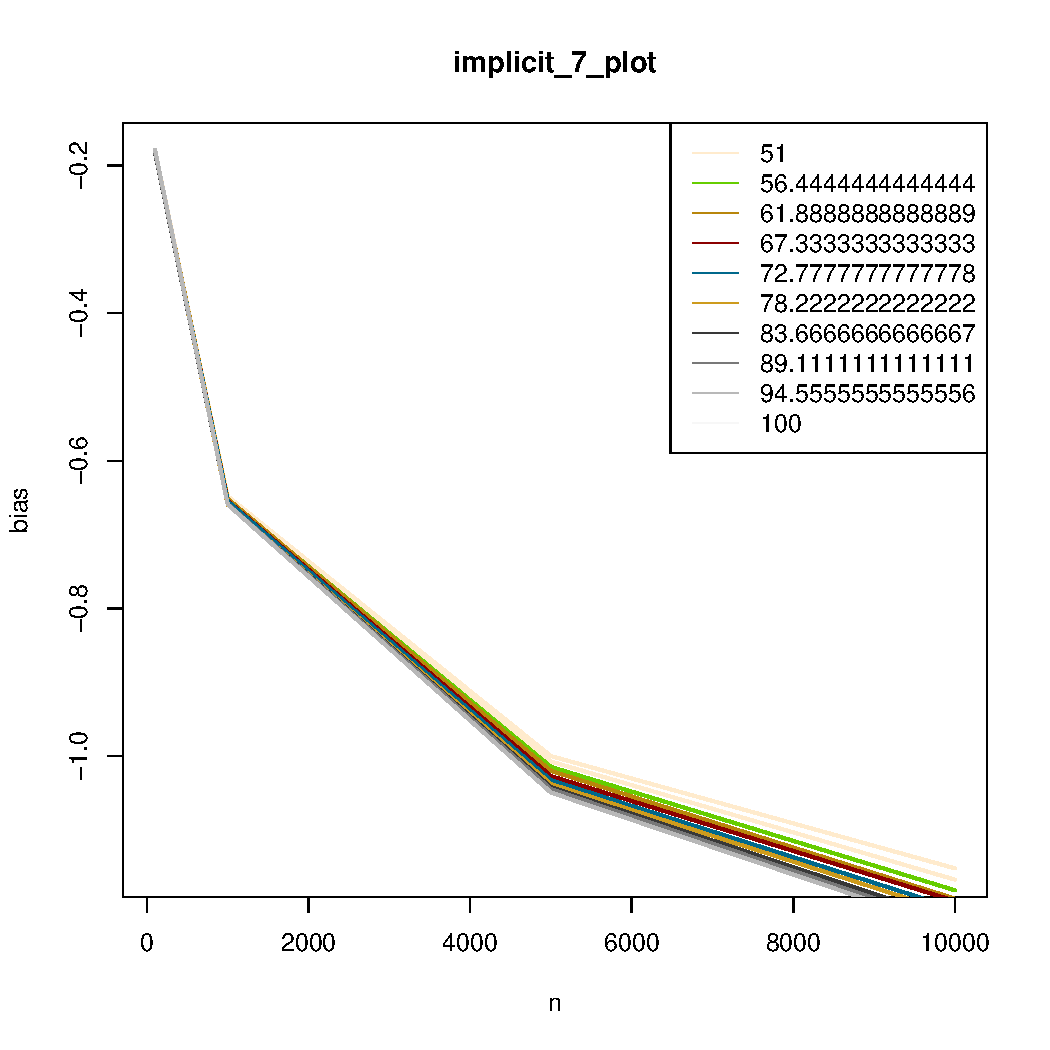
\includegraphics[width=250px]{implicit_7_plot.pdf} \\
        Discussion: Do note that ASGD might be a little off relatively to the other ones because of the learning rate problem we had with 2(b). Regardless, of that looking at the plots of bias over the different $\alpha$ values, we see that it seems that as alpha gets bigger, the bias is relatively smaller. This makes sense because as we have bigger $\alpha$'s we will converge faster because each jump is slightly more powerful.
      \item Trace of the empirical variance plotted on a log scale, from same data as part (c): \\
        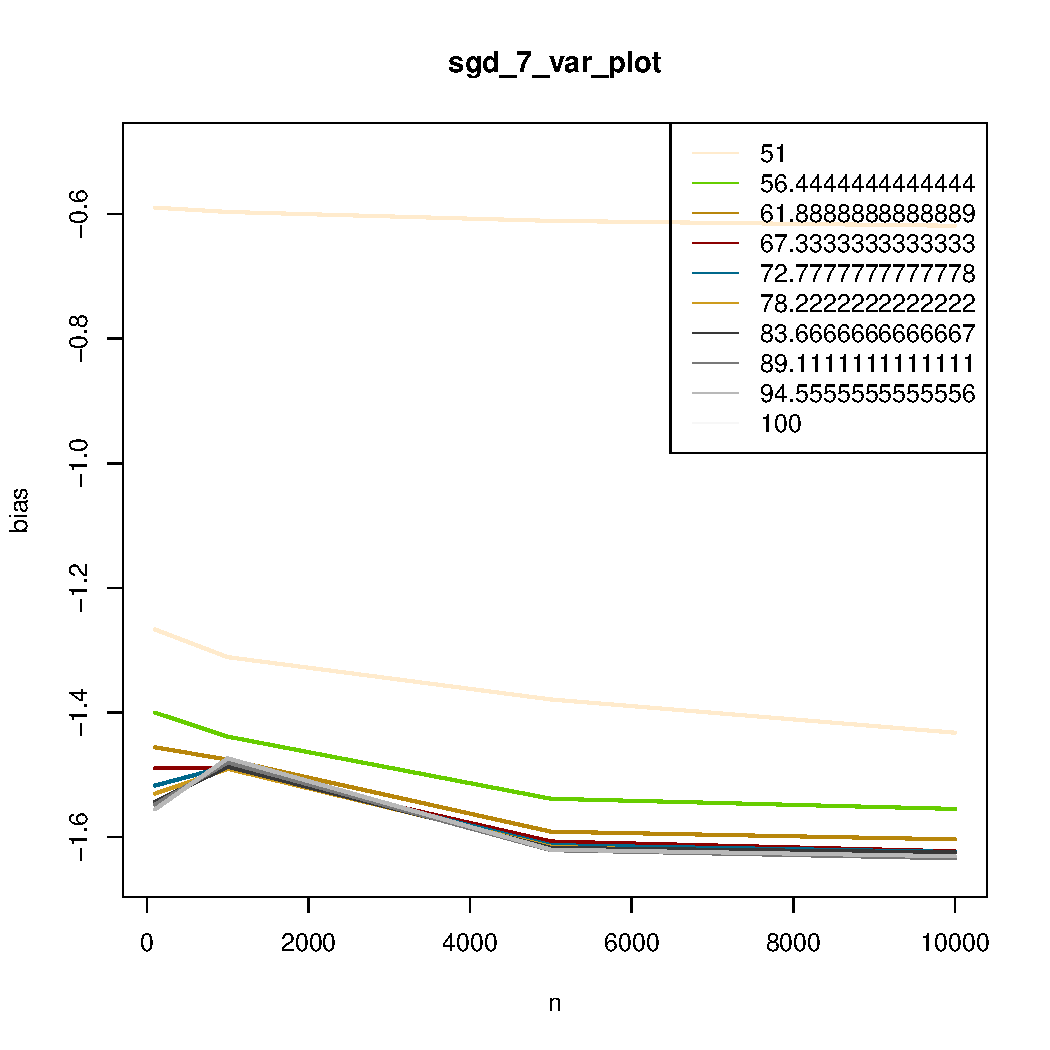
\includegraphics[width=250px, trim=20px 0px 0px 0px, clip=true]{sgd_7_var_plot.pdf} \\
        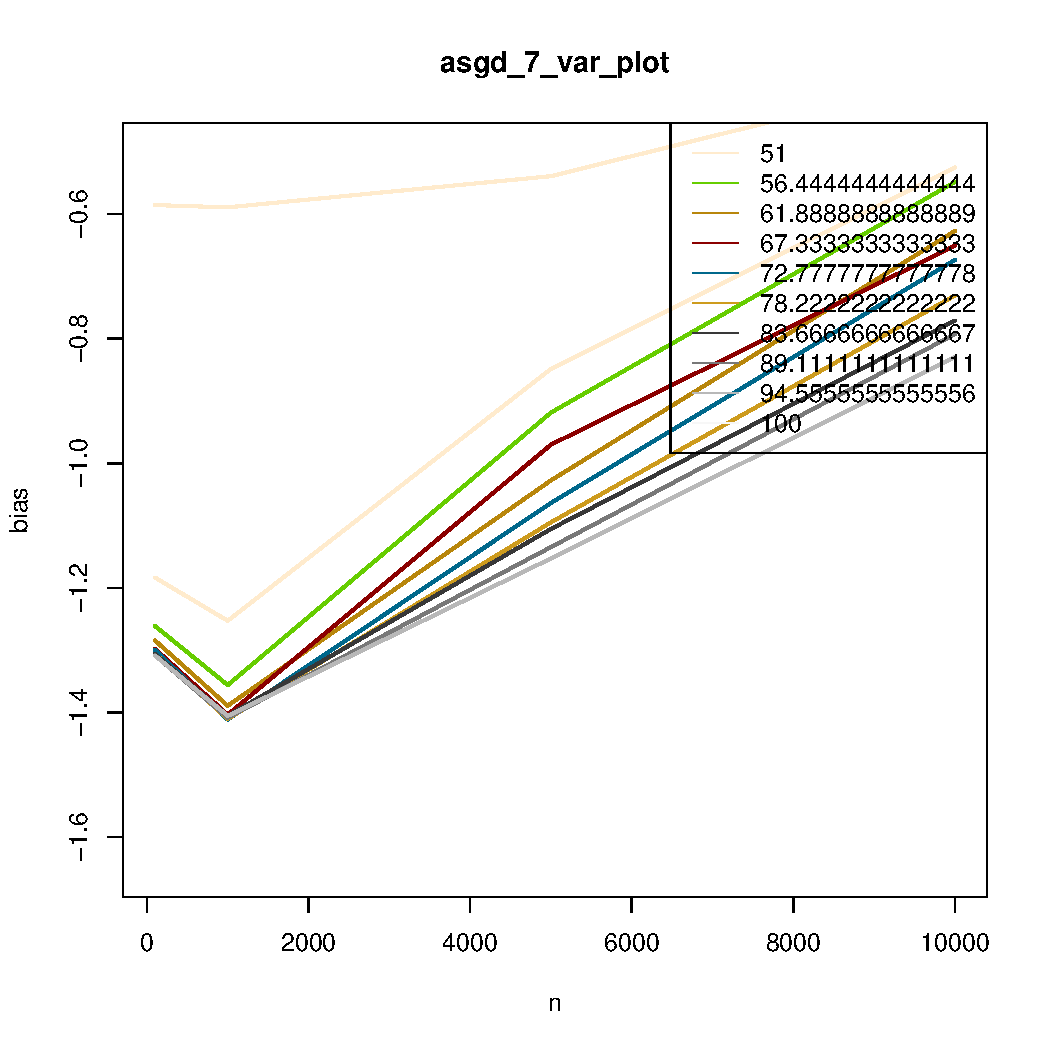
\includegraphics[width=250px, trim=20px 0px 0px 0px, clip=true]{asgd_7_var_plot.pdf} \\
        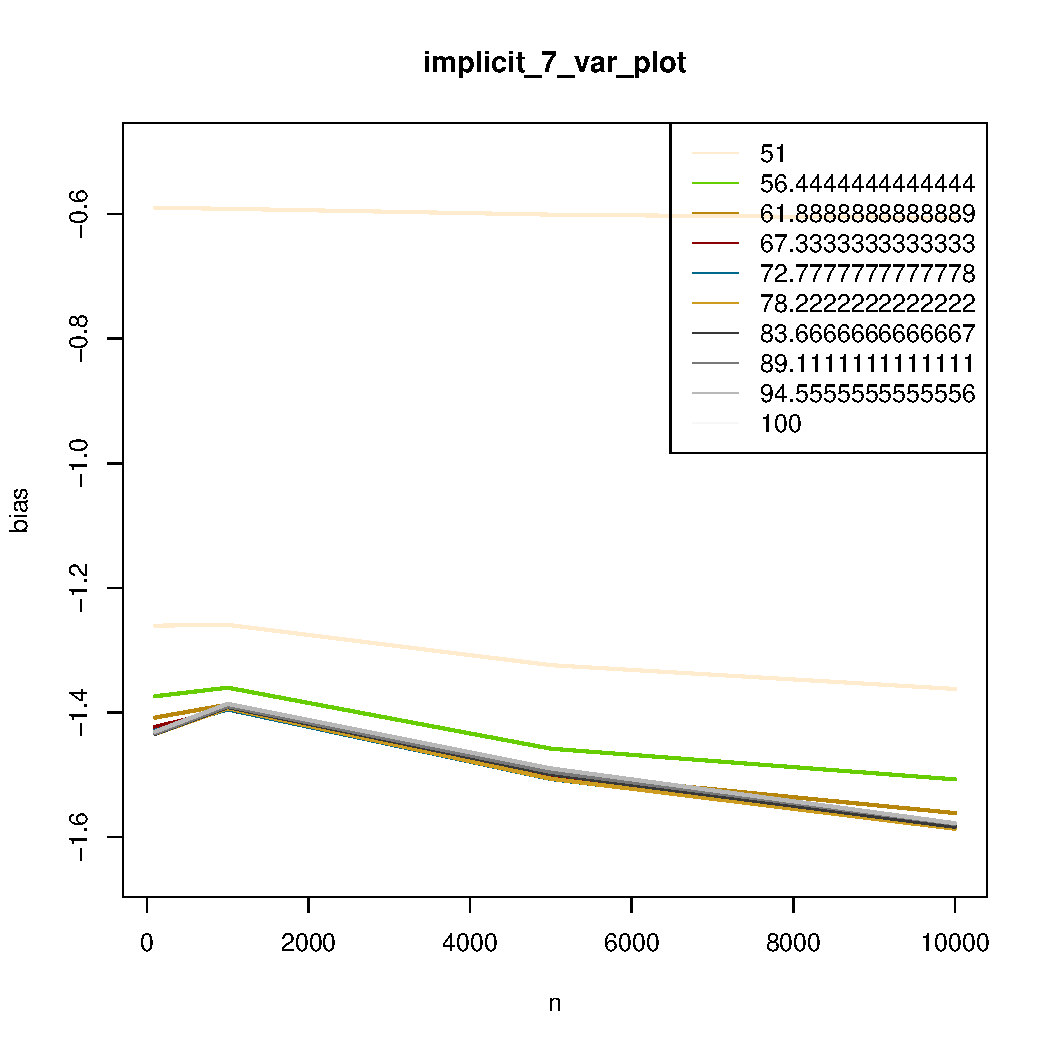
\includegraphics[width=250px, trim=20px 0px 0px 0px, clip=true]{implicit_7_var_plot.pdf} \\
        Discussion: Again, ASGD doesn't seem to follow the same trend as the other charts. It seems that while a small $\alpha = 51$ has a very high variance (probably because it's close to the smallest $\alpha$ value possible), the other values don't really follow a clear trend. For SGD and Implicit, it looks like as we get higher, the variance gets lower until some point at which it stops decreasing.
      \item Yo.
    \end{enumerate}
   \item Part 3
      \begin{table}[!htbp] \centering 
  \caption{N = 1000, p = 100} 
  \label{} 
\begin{tabular}{@{\extracolsep{5pt}} ccccccc} 
\\[-1.8ex]\hline 
\hline \\[-1.8ex] 
 & 0 & 0.1 & 0.2 & 0.5 & 0.9 & 0.95 \\ 
\hline \\[-1.8ex] 
glmnet (type = "naive") & $0.035$ & $0.037$ & $0.041$ & $0.058$ & $0.144$ & $0.249$ \\ 
glmnet (type = "cov") & $0.010$ & $0.011$ & $0.011$ & $0.011$ & $0.017$ & $0.021$ \\ 
lars & $0.210$ & $0.207$ & $0.216$ & $0.214$ & $0.210$ & $0.213$ \\ 
\hline \\[-1.8ex] 
\end{tabular} 
\end{table}   
%MSE table1

	  \begin{table}[!htbp] \centering 
  \caption{N = 5000, p = 100} 
  \label{} 
\begin{tabular}{@{\extracolsep{5pt}} ccccccc} 
\\[-1.8ex]\hline 
\hline \\[-1.8ex] 
 & 0 & 0.1 & 0.2 & 0.5 & 0.9 & 0.95 \\ 
\hline \\[-1.8ex] 
glmnet (type = "naive") & $0.129$ & $0.129$ & $0.148$ & $0.192$ & $0.480$ & $0.804$ \\ 
glmnet (type = "cov") & $0.033$ & $0.034$ & $0.032$ & $0.035$ & $0.038$ & $0.039$ \\ 
lars & $1.023$ & $1.053$ & $1.036$ & $1.047$ & $1.038$ & $1.029$ \\ 
\hline \\[-1.8ex] 
\end{tabular} 
\end{table}

	  \begin{table}[!htbp] \centering 
  \caption{N = 100, p = 1000} 
  \label{} 
\begin{tabular}{@{\extracolsep{5pt}} ccccccc} 
\\[-1.8ex]\hline 
\hline \\[-1.8ex] 
 & 0 & 0.1 & 0.2 & 0.5 & 0.9 & 0.95 \\ 
\hline \\[-1.8ex] 
glmnet (type = "naive") & $0.026$ & $0.024$ & $0.025$ & $0.030$ & $0.048$ & $0.051$ \\ 
glmnet (type = "cov") & $0.047$ & $0.045$ & $0.051$ & $0.070$ & $0.151$ & $0.136$ \\ 
lars & $0.319$ & $0.296$ & $0.303$ & $0.288$ & $0.306$ & $0.327$ \\ 
\hline \\[-1.8ex] 
\end{tabular} 
\end{table}    
   
	   \begin{table}[!htbp] \centering 
  \caption{N = 100, p = 5000} 
  \label{} 
\begin{tabular}{@{\extracolsep{5pt}} ccccccc} 
\\[-1.8ex]\hline 
\hline \\[-1.8ex] 
 & 0 & 0.1 & 0.2 & 0.5 & 0.9 & 0.95 \\ 
\hline \\[-1.8ex] 
glmnet (type = "naive") & $0.073$ & $0.075$ & $0.073$ & $0.086$ & $0.110$ & $0.194$ \\ 
glmnet (type = "cov") & $0.237$ & $0.257$ & $0.256$ & $0.312$ & $0.655$ & $0.679$ \\ 
lars & $1.893$ & $1.658$ & $1.619$ & $1.694$ & $1.758$ & $1.578$ \\ 
\hline \\[-1.8ex] 
\end{tabular} 
\end{table}    
   
		\begin{table}[!htbp] \centering 
  \caption{N = 100, p = 20000} 
  \label{} 
\begin{tabular}{@{\extracolsep{5pt}} ccccccc} 
\\[-1.8ex]\hline 
\hline \\[-1.8ex] 
 & 0 & 0.1 & 0.2 & 0.5 & 0.9 & 0.95 \\ 
\hline \\[-1.8ex] 
glmnet (type = "naive") & $0.264$ & $0.268$ & $0.269$ & $0.288$ & $0.347$ & $0.528$ \\ 
glmnet (type = "cov") & $0.981$ & $1.034$ & $1.069$ & $1.267$ & $2.348$ & $2.777$ \\ 
lars & $6.854$ & $7.487$ & $7.398$ & $7.351$ & $8.118$ & $7.584$ \\ 
\hline \\[-1.8ex] 
\end{tabular} 
\end{table}    

		\begin{table}[!htbp] \centering 
  \caption{N = 100, p = 50000} 
  \label{} 
\begin{tabular}{@{\extracolsep{5pt}} ccccccc} 
\\[-1.8ex]\hline 
\hline \\[-1.8ex] 
 & 0 & 0.1 & 0.2 & 0.5 & 0.9 & 0.95 \\ 
\hline \\[-1.8ex] 
glmnet (type = "naive") & $0.657$ & $0.714$ & $0.731$ & $0.722$ & $0.839$ & $1.598$ \\ 
glmnet (type = "cov") & $2.566$ & $2.666$ & $2.536$ & $3.227$ & $6.326$ & $8.347$ \\ 
lars & $22.491$ & $22.561$ & $25.666$ & $25.018$ & $23.115$ & $24.605$ \\ 
\hline \\[-1.8ex] 
\end{tabular} 
\end{table}    



%Part 3.C
\begin{table}[!htbp] \centering 
  \caption{N = 1000, p = 100} 
  \label{} 
\begin{tabular}{@{\extracolsep{5pt}} ccccccc} 
\\[-1.8ex]\hline 
\hline \\[-1.8ex] 
 & 0 & 0.1 & 0.2 & 0.5 & 0.9 & 0.95 \\ 
\hline \\[-1.8ex] 
SGD Time & $0.261$ & $0.263$ & $0.258$ & $0.276$ & $0.266$ & $0.268$ \\ 
Implicit SGD Time & $0.246$ & $0.246$ & $0.245$ & $0.248$ & $0.251$ & $0.250$ \\ 
SGD MSE & $0.147$ & $0.157$ & $0.148$ & $0.168$ & $0.163$ & $0.154$ \\ 
Implicit SGD MSE & $0.129$ & $0.132$ & $0.133$ & $0.133$ & $0.142$ & $0.139$ \\ 
\hline \\[-1.8ex] 
\end{tabular} 
\end{table} 

\begin{table}[!htbp] \centering 
  \caption{N = 5000, p = 100} 
  \label{} 
\begin{tabular}{@{\extracolsep{5pt}} ccccccc} 
\\[-1.8ex]\hline 
\hline \\[-1.8ex] 
 & 0 & 0.1 & 0.2 & 0.5 & 0.9 & 0.95 \\ 
\hline \\[-1.8ex] 
SGD Time & $5.486$ & $5.540$ & $5.665$ & $5.529$ & $5.539$ & $5.620$ \\ 
Implicit SGD Time & $5.476$ & $5.516$ & $5.605$ & $5.563$ & $5.617$ & $5.577$ \\ 
SGD MSE & $4.421$ & $4.342$ & $4.275$ & $4.133$ & $4.150$ & $4.187$ \\ 
Implicit SGD MSE & $4.399$ & $4.274$ & $4.162$ & $4.136$ & $4.151$ & $4.192$ \\ 
\hline \\[-1.8ex] 
\end{tabular} 
\end{table} 

\begin{table}[!htbp] \centering 
  \caption{N = 100, p = 1000} 
  \label{} 
\begin{tabular}{@{\extracolsep{5pt}} ccccccc} 
\\[-1.8ex]\hline 
\hline \\[-1.8ex] 
 & 0 & 0.1 & 0.2 & 0.5 & 0.9 & 0.95 \\ 
\hline \\[-1.8ex] 
SGD Time & $1.643$ & $1.607$ & $1.623$ & $1.617$ & $1.617$ & $1.631$ \\ 
Implicit SGD Time & $1.602$ & $1.623$ & $1.629$ & $1.622$ & $1.631$ & $1.659$ \\ 
SGD MSE & $0.037$ & $0.036$ & $0.040$ & $0.039$ & $0.039$ & $0.035$ \\ 
Implicit SGD MSE & $0.035$ & $0.037$ & $0.043$ & $0.040$ & $0.040$ & $0.035$ \\ 
\hline \\[-1.8ex] 
\end{tabular} 
\end{table}

\begin{table}[!htbp] \centering 
  \caption{N = 100, p = 5000} 
  \label{} 
\begin{tabular}{@{\extracolsep{5pt}} ccccccc} 
\\[-1.8ex]\hline 
\hline \\[-1.8ex] 
 & 0 & 0.1 & 0.2 & 0.5 & 0.9 & 0.95 \\ 
\hline \\[-1.8ex] 
SGD Time & $172.810$ & $172.320$ & $172.874$ & $172.882$ & $172.961$ & $174.794$ \\ 
Implicit SGD Time & $172.752$ & $175.411$ & $175.180$ & $177.150$ & $175.977$ & $177.233$ \\ 
SGD MSE & $0.820$ & $0.827$ & $0.881$ & $0.865$ & $0.881$ & $0.831$ \\ 
Implicit SGD MSE & $0.809$ & $0.867$ & $0.938$ & $0.993$ & $1.004$ & $0.910$ \\ 
\hline \\[-1.8ex] 
\end{tabular} 
\end{table} 

%MSE Tables for GLMnet
	\begin{table}[!htbp] \centering 
  \caption{MSEs: N = 1000, p = 100} 
  \label{} 
\begin{tabular}{@{\extracolsep{5pt}} ccccccc} 
\\[-1.8ex]\hline 
\hline \\[-1.8ex] 
 & 0 & 0.1 & 0.2 & 0.5 & 0.9 & 0.95 \\ 
\hline \\[-1.8ex] 
glmnet (type = "naive") & $0.045$ & $0.045$ & $0.045$ & $0.048$ & $0.057$ & $0.080$ \\ 
glmnet (type = "cov") & $0.039$ & $0.044$ & $0.040$ & $0.044$ & $0.062$ & $0.072$ \\ 
\hline \\[-1.8ex] 
\end{tabular} 
\end{table} 

	\begin{table}[!htbp] \centering 
  \caption{MSEs: N = 5000, p = 100} 
  \label{} 
\begin{tabular}{@{\extracolsep{5pt}} ccccccc} 
\\[-1.8ex]\hline 
\hline \\[-1.8ex] 
 & 0 & 0.1 & 0.2 & 0.5 & 0.9 & 0.95 \\ 
\hline \\[-1.8ex] 
glmnet (type = "naive") & $0.028$ & $0.027$ & $0.028$ & $0.030$ & $0.050$ & $0.070$ \\ 
glmnet (type = "cov") & $0.027$ & $0.028$ & $0.028$ & $0.029$ & $0.051$ & $0.068$ \\ 
\hline \\[-1.8ex] 
\end{tabular} 
\end{table} 

	\begin{table}[!htbp] \centering 
  \caption{MSEs: N = 100, p = 1000} 
  \label{} 
\begin{tabular}{@{\extracolsep{5pt}} ccccccc} 
\\[-1.8ex]\hline 
\hline \\[-1.8ex] 
 & 0 & 0.1 & 0.2 & 0.5 & 0.9 & 0.95 \\ 
\hline \\[-1.8ex] 
glmnet (type = "naive") & $0.064$ & $0.060$ & $0.063$ & $0.060$ & $0.067$ & $0.071$ \\ 
glmnet (type = "cov") & $0.062$ & $0.064$ & $0.064$ & $0.057$ & $0.064$ & $0.069$ \\ 
\hline \\[-1.8ex] 
\end{tabular} 
\end{table}

	\begin{table}[!htbp] \centering 
  \caption{MSEs: N = 100, p = 5000} 
  \label{} 
\begin{tabular}{@{\extracolsep{5pt}} ccccccc} 
\\[-1.8ex]\hline 
\hline \\[-1.8ex] 
 & 0 & 0.1 & 0.2 & 0.5 & 0.9 & 0.95 \\ 
\hline \\[-1.8ex] 
glmnet (type = "naive") & $0.033$ & $0.031$ & $0.032$ & $0.031$ & $0.030$ & $0.032$ \\ 
glmnet (type = "cov") & $0.030$ & $0.033$ & $0.029$ & $0.030$ & $0.032$ & $0.031$ \\ 
\hline \\[-1.8ex] 
\end{tabular} 
\end{table} 

	\begin{table}[!htbp] \centering 
  \caption{MSEs: N = 100, p = 20000} 
  \label{} 
\begin{tabular}{@{\extracolsep{5pt}} ccccccc} 
\\[-1.8ex]\hline 
\hline \\[-1.8ex] 
 & 0 & 0.1 & 0.2 & 0.5 & 0.9 & 0.95 \\ 
\hline \\[-1.8ex] 
glmnet (type = "naive") & $0.016$ & $0.017$ & $0.015$ & $0.016$ & $0.016$ & $0.017$ \\ 
glmnet (type = "cov") & $0.017$ & $0.017$ & $0.016$ & $0.017$ & $0.017$ & $0.017$ \\ 
\hline \\[-1.8ex] 
\end{tabular} 
\end{table} 

	\begin{table}[!htbp] \centering 
  \caption{MSEs: N = 100, p = 50000} 
  \label{} 
\begin{tabular}{@{\extracolsep{5pt}} ccccccc} 
\\[-1.8ex]\hline 
\hline \\[-1.8ex] 
 & 0 & 0.1 & 0.2 & 0.5 & 0.9 & 0.95 \\ 
\hline \\[-1.8ex] 
glmnet (type = "naive") & $0.010$ & $0.011$ & $0.011$ & $0.011$ & $0.011$ & $0.010$ \\ 
glmnet (type = "cov") & $0.010$ & $0.010$ & $0.010$ & $0.011$ & $0.011$ & $0.010$ \\ 
\hline \\[-1.8ex] 
\end{tabular} 
\end{table} 

\end{enumerate}
\end{document}
